\chapter{Introduction}
\label{sec:intro}

Better transmission performance has been an ever-lasting pursuit of network engineers and researchers since the dawn of Internet. 
%The pursuit is stemmed from the distributed routing behavior that ensures the prevalence of this collection of individually manged networks.
With in the realm of Internet, networks and hosts alike selfishly compete for resources on common parts of paths.
Such behavior gives rise to congestion and sub-optimal traffic distribution from a global view.

Congestion takes place on an Internet path shared by multiple flows when the total demand exceeds the link capacity.
Avoiding vicious competition that eventually blocks all flows, end-to-end congestion control mechanism plays an important role. It improves transmission performance in a distributed manner.
It aims at 1) fully utilizing bottleneck bandwidth while 2) introducing minimum additional transmission delay (short queue length) and 3) ensuring fair share of resources~\cite{Jacobson1988, mathis1997macroscopic, Cardwell2016}.

The transmission performance can be further improved with big enough link capacity to satisfy the demand of all flows. To that end, it is necessary to regularly dimension the network according to the growth of traffic demands~\cite{pioro2004routing}. 
%Among all the sections of Internet, access network has a notorious reputation as bottleneck.
%Over last years, new generations of access methods~\cite{Kramer2002, kazovsky2007next} have greatly enlarged the pipe of this `last mile'. 
Yet, infrastructure-building alone is not enough. First, network deployment happens on a much longer time span than traffic fluctuations. Before extra capacity is deployed, some links may become saturated while others remain almost idle, due to changes in traffic demand. Second, over-dimensioning is costly, given that future technologies will drastically reduce the cost per bandwidth unit.

Therefore, reactive and flexible routing schemes are needed, complementary to network dimensioning.
They maximize the actual usable capacity.
Within a network (intradomain), the administrator may in first place estimate/shape the traffic matrix 
that comes across its network. Then, each flow can be split onto multiple paths to best fit in the available capacity~\cite{Xu2011, Jain2013}.
Across different networks (interdomain), the room for performance improvement comes mainly from multiple Internet paths between source and destination networks.
It is because the end-to-end bottleneck capacity is potentially enlarged with richer Internet paths.
Such path diversity can already be obtained through multihoming under current \acf{BGP}. With multihoming, a network purchases the access to the rest of the Internet via multiple providers. Many other propositions as well encourage the propagation of multiple Internet paths, to name a few BGP Add-path~\cite{addpath}, MIRO~\cite{Xu2006}, NIRA~\cite{Yang2007}, YAMR~\cite{Ganichev2010}, Pathlet routing~\cite{Godfrey09}, IDRD~\cite{Misseri2013}, and etc.
However, in interdomain routing, each network generally does not have the visibility outside its own territory, e.g. capacity of a remote link and competing traffic demand from other networks on that link.
This is particularly true with \ac{BGP}, the de facto interdomain routing protocol that is not going to obsolete shortly.
Therefore, it is not possible for current networks to figure out which available paths offer the best performance toward a certain destination.
In other words, the challenge is how to make better use of available Internet capacity with a performance agnostic protocol \ac{BGP}.
We undertake this challenge in this dissertation.

One straightforward way to make the route decision performance-aware is through measurement. In engineering their interdomain peering edge, both Facebook and Google employ instrumentation embedded in their applications to learn end-to-end performance over multiple available paths~\cite{Yap2017, Schlinker2017}.
As transit price drops, multihoming becomes rather a common practice of numerous medium and small size networks. 
These networks as well have the immediate need for performance improvements, so that their business could survive.

Despite the concrete need for measurement-based interdomain traffic engineering, many questions remain unanswered, or partially addressed.
A typical network can communicate with $\sim$ 100k different destinations regularly. 
Continuously measuring the performance to all that many destinations are costly and not necessary. 
What are the most important destinations to focus on? Do these destinations change over time? How to identify them?
Besides volume measurements, how should performance measurements be processed? Do they need cleaning?
If yes, what are the potential data quality issues? What are the origins of these issues? How can we showcase and mitigate their impacts on route selection?
Further, in order to dynamically react to performance changes, how to detect in first place significant changes in performance measurements? How to do so without hard-coded or ad hoc parameters? How to achieve at meantime an acceptable level of robustness?
Finally, once a performance change is detected, how can we learn more about this event from a network perspective? Where does it happen? Does it potentially impact other Internet paths currently in use? 
We aim to explore answers to the above questions in this dissertation, so that the building of measurement-based route selection system advances in these aspects: measurement scalability, interpretation of performance data and visibility on causes of performance changes. 

\chapter{Background, scope and roadmap}
\section{Intradomain Routing}
\begin{figure}[!htb]
\centering
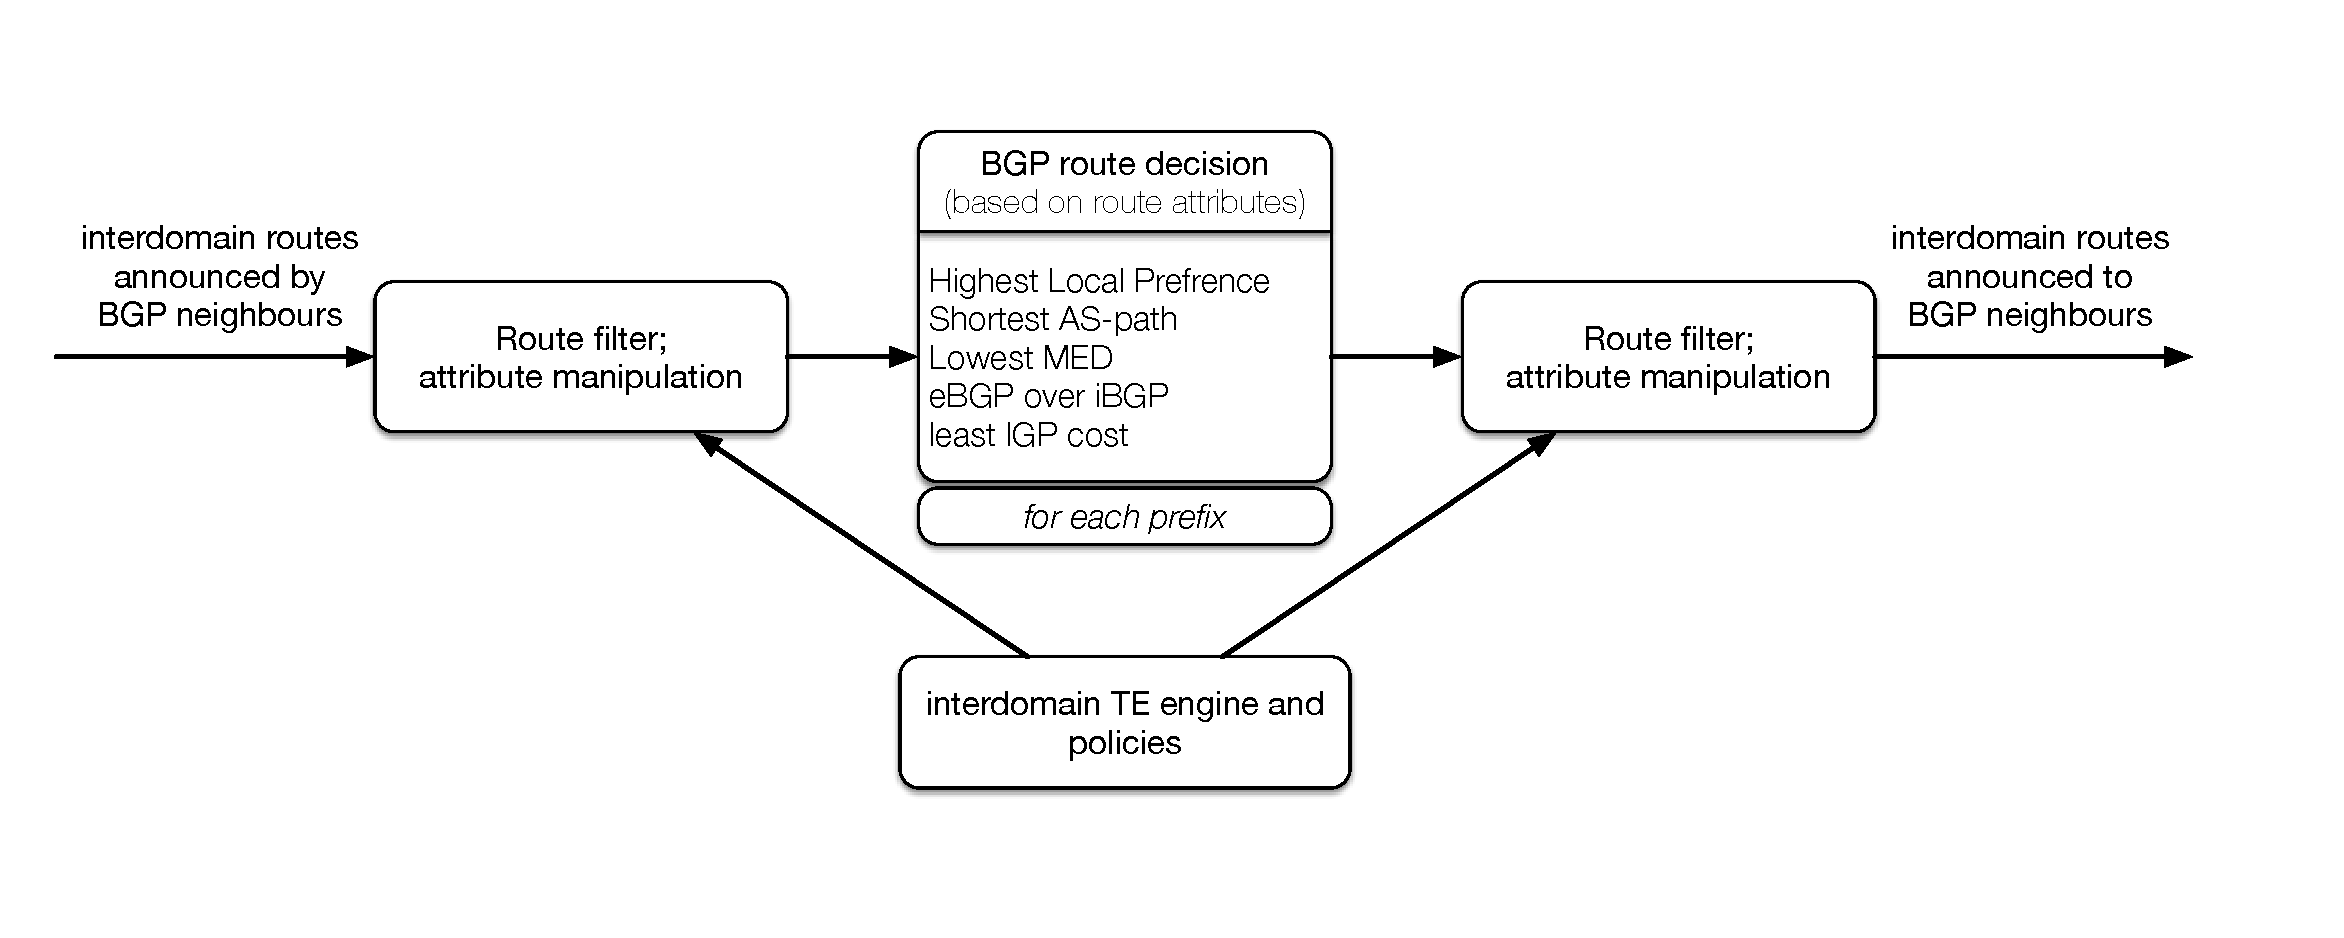
\includegraphics[width=1.3\textwidth]{gfx/chap1/bgp_decision.pdf}
\caption{Workflow of \acf{BGP} route selection and propagation within an \acf{AS}.}
\label{fig:bgp_decision}
\end{figure}

Interconnection of tens of thousands of independently manged networks forms Internet.
Each individual network is as well called an \acf{AS}.
Routing that happens among those ASes is referred to as 
\textit{interdomain routing}.
In order to exchange interdomain routes, each AS uses \acf{BGP}~\cite{bgp4}, a path vector routing protocol, to communicate with other ASes.
Each AS announces its own routes (routes towards its own prefixes) along with other routes to its BGP neighbors.
For each prefix as destination, one single best route is selected by the BGP route decision process.
The selection considers the BGP attributes attached to each route, as illustrated in Figure.~\ref{fig:bgp_decision}.
According to configured TE polices, each route can be filtered or altered based on its attributes~\cite{Quoitin2003, Gao2001a}.
Such operations can take place before BGP route decision and as well before route advertisement to its neighbors.

\begin{figure}[!htb]
\centering
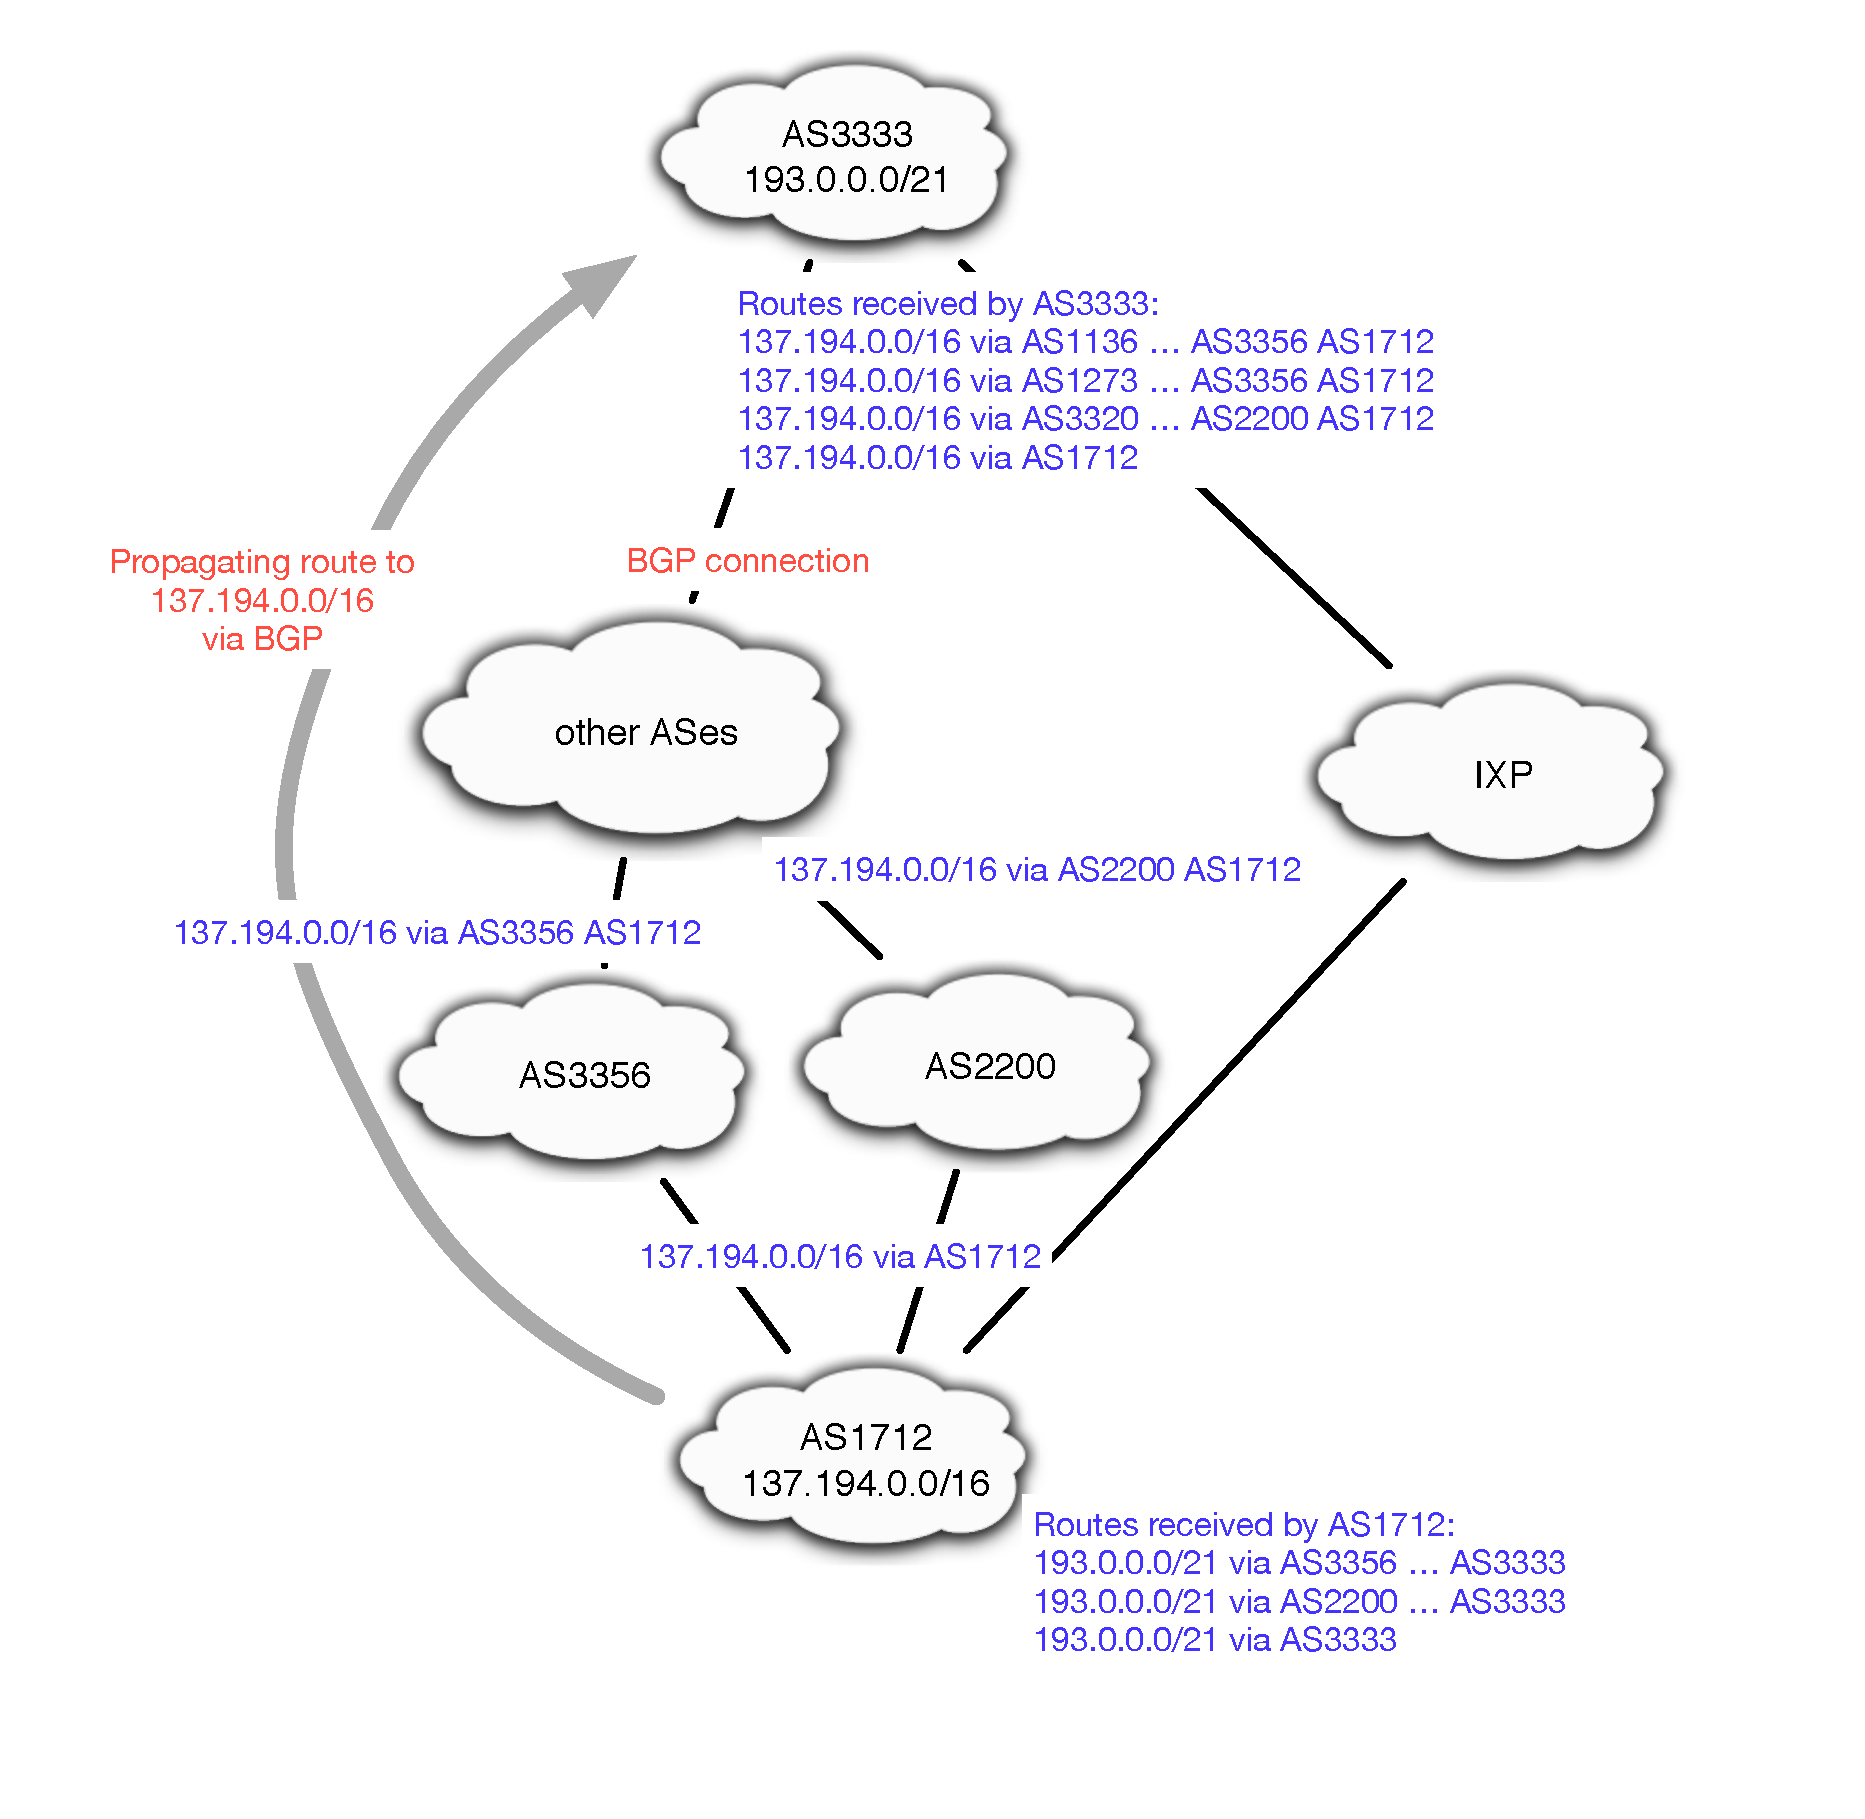
\includegraphics[width=1.1\textwidth]{gfx/chap1/bgp_route_propagation.pdf}
\caption{Interdomain route propagation via \ac{BGP}, an example of \texttt{137.194.0.0/16}. Networks illustrated are fictional.}
\label{fig:bgp_propa}
\end{figure}

Fig.~\ref{fig:bgp_propa} illustrates the propagation of interdomain routes to prefix \texttt{137.194.0.0/16} of AS1712 via BGP exchanges. Each AS inserts its own AS number when announcing the route to other ASes, thus forming an AS path at the receiver side. After AS3333 learns the routes to \texttt{137.194.0.0/16} and AS1712 learns routes to \texttt{193.0.0.0/21} in a similar way, the two ASes can exchange traffic across Internet using these two prefixes.

There are two types of ASes in the above BGP exchanges: \textit{transit provider} and \textit{stub AS}.
Transit provider refers to ASes that offer to route traffic not originated from nor sent to itself, as a commercial service.
For that purpose, a transit provider announces to its clients all the interdomain routes its learns and to its other BGP neighbors the routes to its clients.
In Figure~\ref{fig:bgp_propa}, AS3356 and AS2200 are transit providers of AS1712. They help announce the route to prefix \texttt{137.194.0.0/16}
to the rest of Internet.
On the contrary, a stub AS only cares about sending out its own traffic and becoming reachable to others.
Accordingly, it only announces to its transit providers its own routes. 
AS1712 is a stub AS in Figure~\ref{fig:bgp_propa}, as it does not relay interdomain routes for other ASes. For example, AS1712 will not announce to AS3356 the route to \texttt{193.0.0.0/21} learnt from AS2200. Consequently no traffic toward ASes other than itself shall arrive at it.

Besides the relationship described above, peering is another type of exchange under BGP. Two ASes in peering relationship exchange with each other their own routes, so that they can directly communicate without employing a transit provider.
In Figure~\ref{fig:bgp_propa}, AS1712 and AS3333 directly peer at an \ac{IXP}.
\ac{IXP} is a collocation facility that eases establishment of peering relationship, thus is transparent to BGP route exchanges.

\section{Interdomain TE}
Thanks to transit and peering relationship, AS3333 and AS1712 in Figure~\ref{fig:bgp_propa} may receive multiple routes to send out traffic.
Meanwhile, they may as well receive traffic from multiple neighbors.
Such diversity in route brings up two questions: 1) which routes are the best; 2) how to route corresponding traffic on the desired paths.
The efforts spared in answering these two questions are referred to as \textit{interdomain \ac{TE}}~\cite{Quoitin2004a,Quoitin2003,Feamster2003}.

The first question deals with the objective of \ac{TE}. In general, a network aims at optimizing the cost and/or performance of transmission.
The second question explores the method to steer traffic.
We summarize the current practices, their limitations and challenges for incoming and outgoing traffic separately in this section.

\subsection{Outbound interdomain TE}
%Outbound TE consists in 1) how to identify the best routes for each destination prefix and send out the traffic on these routes 
In sending traffic to a destination prefix, an AS has total control over the routes to be employed. One One common practice is to tune \textit{local preference} BGP attributes~\cite{Wang2008} before BGP route decision (Figure~\ref{fig:bgp_decision}). 
Therefor the challenge is rather on the composition of best routes in terms of cost and performance.

The cost of interdomain transmission depends on the the $95^th$ percentile bandwidth consumption on links purchased from transit providers, i.e. transit links~\cite{drpeering-95th}.
Meanwhile, whether these transit links are congested impacts in return the transmission performance.
Hence, outbound TE resolves in dynamically calculating the appropriate amount of traffic to be routed on each transit link.
The objective of such traffic re-distribution is to lower the overall transit cost, under the constraint of not saturating any transit link at any instant (if possible).

\citet{Goldenberg2004} formulated this quest as a minimum-cost multi-commodity flow problem.
\citet{Uhlig2004b} fulfills the same goal while minimizing the number of route changes by predicting the traffic volume.
\citet{Zhu2014} avoids congestion on transit links by including border router queue length in route decision.

Performance-wise, it is clearly sub-optimal to greedily saturate the cheapest transit link while other transit links remain idle.
However, there are other factors that may as well put transmission performance in danger.
The minimum delay of Internet transmission is dominated by the physical length traversed by a route. 
However, neither AS path length nor transit cost reveals/correlates to the underlying distance.
On top of that, transient events like congestion can as well happen remotely~\cite{Akella2003, Luckie2014}, independent of traffic load on transit links.
To identify performance difference across multiple routes, end-to-end measurements are indispensable.
They cumulatively reflect the contribution along the entire path, including the transit links.


\subsection{Inbound interdomain TE}
Inbound TE takes care of the incoming traffic distribution on available transit links.
Through Figure~\ref{fig:bgp_decision} and \ref{fig:bgp_propa}, we learn that the paths that incoming traffic takes are decided by remote senders.
For instance, AS3333 decides which routes to use to send traffic to \texttt{137.194.0.0/16} of AS1712.
What AS1712 can do to influence the the route decision of AS3333 is to control its route advertisement.
Shown in Figure ~\ref{fig:bgp_decision}, an AS can filter routes or change certain BGP attributes before advertisement.
Some common practices are: selective announcement, more specific announcement, AS path prepending, setting \ac{MED}~\cite{Wang2008}.

These approaches are not perfect. 
Selective announcement introduces reachability risks.
More specific announcement gives rise to \ac{RIB} inflation. 
AS path prepending is shown to be feeble in avoiding a specific ingress link~\cite{Quoitin2004a}. 
BGP community~\cite{Donnet2008, Shao2015} and redistributed communities~\cite{Quoitin2002} allow finer grained operations with better certainty. 
However, it requires the support from transit providers. 

Under BGP, it appears to be very difficult to have a fine control over the paths/ingress links of incoming traffic. 
In this context, many efforts were focused on incoming traffic steering mechanism.
Traffic ingress point can be dictated by setting the source address of outbound traffic to that of the desired ingress interface.
Such address `spoofing' can be achieved through encapsulation~\cite{Liu2008} or \ac{NAT}~\cite{Sun2015}. However, outgoing traffic could be dropped, for security considerations.
Because it seems to come from outside the prefixes that the AS announces\cite{filtering}.
\ac{LISP} pushes such approach to a revolutionary level by introducing a separate addressing space in the core of Internet that enables various TE operations that are impossible with mere BGP~\cite{lisp}. Studies show fine-grained and dynamic inbound optimization is feasible with \ac{LISP}~\cite{Iannone2007, saucez2011mechanisms, quoitin2007evaluating}.
Yet, the protocol deployment remains limited.

\subsection{Software Defined Networking and interdomain TE}
Recently, \acf{SDN} brings as well new possibilities to interdomain TE. 
One idea is to delegate the TE tasks of an AS to a third party.
The third party performs route decision and traffic steering in a centralized manner, in accordance to \ac{SDN} design philosophy.
It is advocated that the interdomain TE can hence be done in a more cooperative way.
Since conflicts of interest involving multiple ASes are solved centrally, an overall optimality can be achieved.
\citet{Kotronis2012} advances that such AS clusters under same TE service provider can form and expand in a gradual way thanks to network effect.
\citet{Gupta2014} focuses on the application of \ac{SDN} in a more specific network environment, \ac{IXP}.
The members of an IXP by nature forms a cluster of ASes.
They exchange their routing information along with their TE polices within one centrally managed facility. 
Application specific peering, e.g. only peer for the exchange of video traffic, is made possible under this framework.

\section{Scope of this thesis}
We stage the works of this thesis under BGP, while fully realizing \ac{LISP}, \ac{SDN} and etc. are promising directions to pursuit.
It is because BGP is still going to be the \textit{de facto} routing protocol of Internet in the foreseeable future.
And the deployment of any new routing mechanism must be incremental.
Before the takeover of anything non-BGP,  BGP is what a majority of ASes have to live with. 
There are thus immediate needs for improvements.

We focus on outbound TE in this thesis.
Inbound TE has been shown to be inherently difficult with BGP, due to lack of effective traffic steering method.

We target stub ASes (potentially multi-homed).
It is because \ac{CP}, \ac{HP} and \ac{ISP}, being major network types among stub ASes, are those who need most outbound TE.
Moreover, dynamic route re-selection in those networks will not cast Internet-wide BGP route convergence issues.

Finally, we assume improving transmission performance is nowadays the major motivation for outbound TE.
Routing traffic across Internet now faces fewer monetary constraints thanks to decreasing transit price~\cite{transitprice, drpeering} and high \ac{IXP} growth rate worldwide~\cite{pchixp}.
Instead, through demand for geographical and topological connection diversity~\cite{Chiu2015}, a performance challenge remains to be addressed.

\section{Measurement-based TE and motivations}
BGP route decision mechanism is unaware of the performance characteristics of candidate paths~\cite{Yannuzzi2005}, as shown in Figure~\ref{fig:bgp_decision}.
Yet, the transmission performance toward a destination varies over different interdomain routes.
\citet{Akella2003} pointed out that bandwidth bottleneck can be within certain transit providers or on the links between remote ASes.
This observation suggests that the choice of transit provide is of relevance to transmission performance.
Further, \citet{Akella2003a} revealed a $30\%$ potential performance gain that an AS could achieve with multi-homing.
%\cite{Akella2004} advocates that this gain is not far away from that of overlay networking.

In order to actually realize this performance gain, dynamic route selection based on performance measurements is required, i.e. \textit{measurement-based TE}.
\citet{Akella2008} presented a demo implementation of a measurement-based TE system.
Only 100 destinations are emulated in this work.
This number is far less from the actually scale that a stub AS might face on a daily base. 
In the work, the best route for each destination is chosen based on the \ac{EWMA} of past \acf{RTT} measurements. 
The results show that the best transmission performance over all destinations is achieved when route decision is made upon last single measurement.
However, considering the noisy nature of \ac{RTT} measurements, such a simplistic approach can lead to overwhelmingly frequent path changes. 
Moreover, treating Internet as a blackbox for delay measurements fails to provide useful and sometimes necessary insight into the underlying network events.
These network events, e.g. path changes and congestion, are the actual causes for significant performance degradation and the reasons of route change.

In order to address the above concerns and narrow down the gap between the concept and a working system~\cite{b6}, 
we study in this thesis traffic volume, delay and path measurements to improve the scalability, measurement interpretation and performance visibility of measurement-based interdomain TE.


\section{Roadmap}
\subsection{Building blocks of measurement-based TE}

\begin{figure}[!htb]
\centering
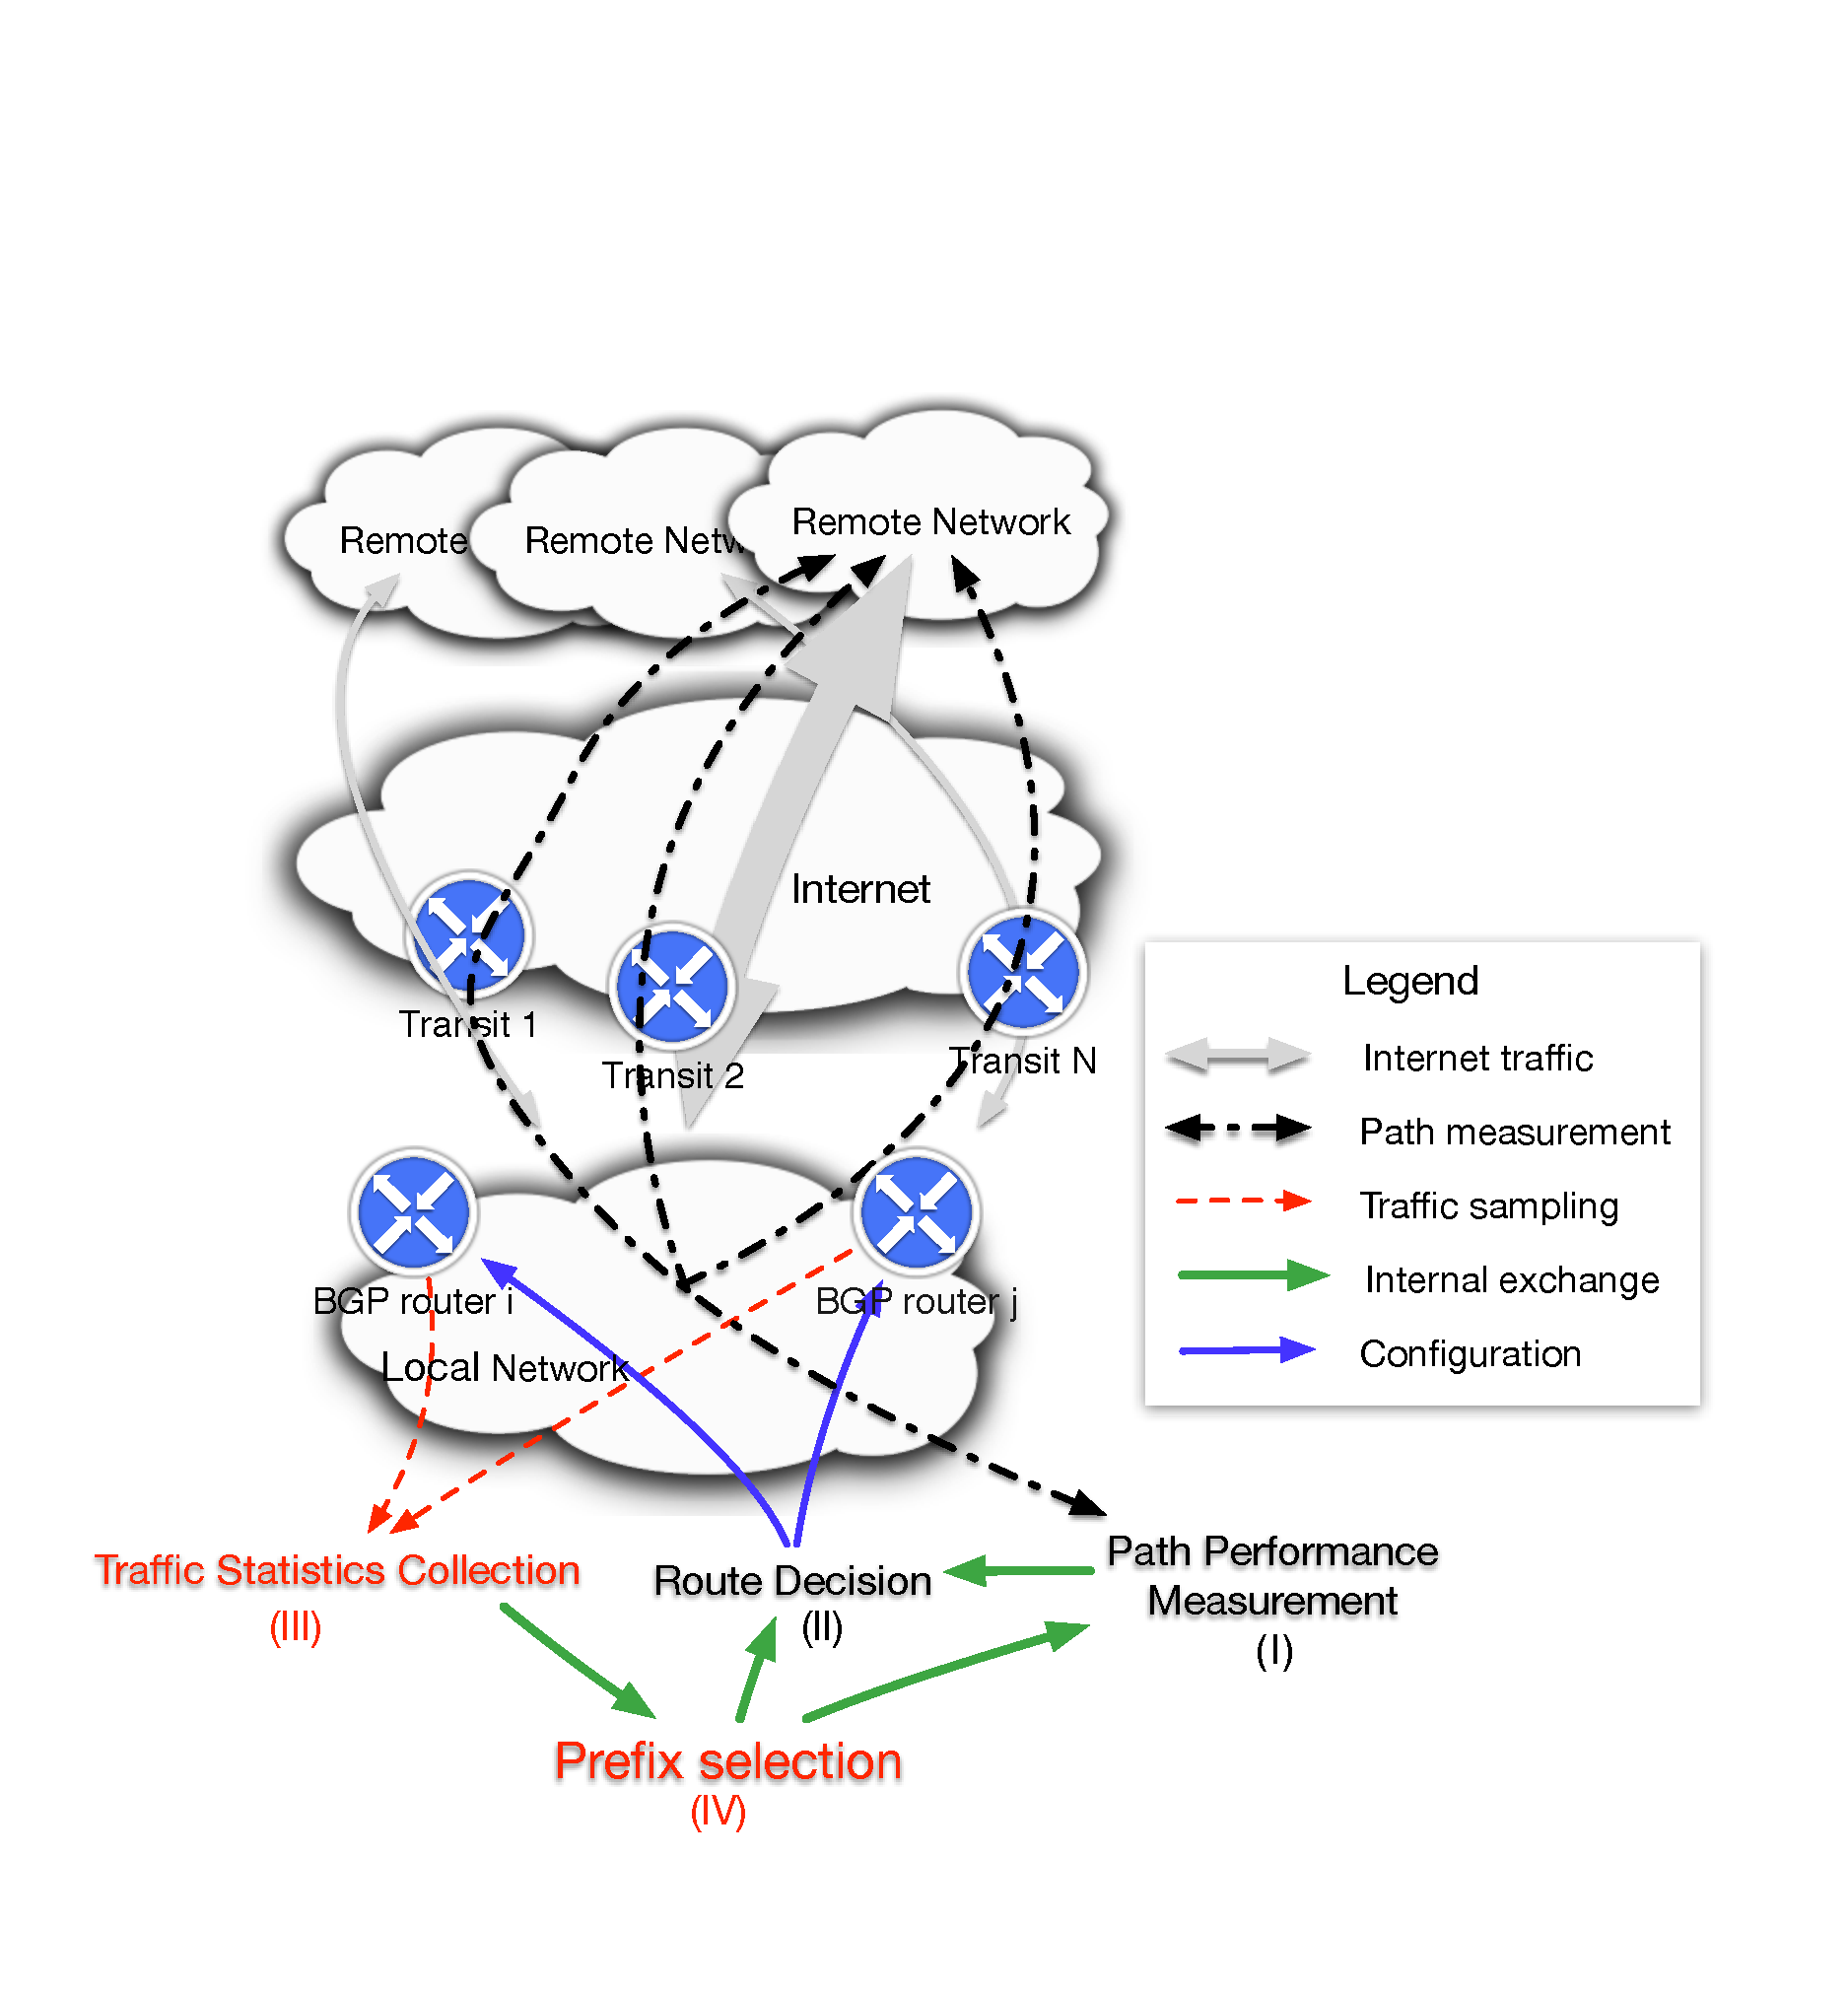
\includegraphics[width=\textwidth]{gfx/chap1/archi.pdf}
\caption{Building blocks of measurement-based inter-domain TE system.}
\label{fig:archi}
\end{figure}

A measurement-based interdomain TE platform has two essential building blocks.
They are illustrated in black in Figure~\ref{fig:archi}: (i) path performance measurement and (ii) route decision.
The platform measures the end-to-end performance, more specifically \acf{RTT}, over all the available routes towards a given destination prefix. 
Within in each destination prefix, a couple of hosts with open ports, e.g. 80, 443, are discovered and then used as probing destination in active delay measurements.
Once fed with performance measurements, route decision engine dictates for each destination the best routes at each moment and imposes them on BGP border routers.

\subsection{Prefix selection: focus on most important destinations}
A scalability issue presents in the above design.
A stub AS can exchange with up to around 100k destination prefixes.
Continuous performance monitoring to all these destinations over all available paths could be prohibitively costly.
\citet{Feamster2003} already realized this issue and proposed to focus on popular destinations.
However, no exact solution was given.
In Chapter~\ref{sec:pref_selec}, we tackle the selection of prefixes associated with important traffic volume.
Through study on their temporal dynamism at different time resolutions, we arrive at very simple yet efficient mechanisms. 
As a part of the proposition, two additional building blocks are added to the system architecture (highlighted in red in Figure~\ref{fig:archi}).

\subsection{RTT measurements with RIPE Atlas}
Studies in Chapter~\ref{sec:pref_selec} base solely on the measurement data collected by a proprietary TE platform~\cite{b6} from client networks. 
Working trace from real networks increases the credibility of our observation. 
However, it brings as well reproducibility concerns.
In Chapter~\ref{sec:ripe_atlas}, we first justify our choice of using RIPE Atlas~\cite{atlas} as source for path and delay measurements in later researches.
We then discuss a data quality issue originated from the measurement platform.

Further, we investigated another data quality issue that is specific to interdomain TE. 
We employ unsupervised learning methods to reveal the inherent structure of a group of delay measurements on a same AS path.

During the above study, we notice an interesting case where several RTT time series exclusively share a similar shape at about the same moment.
We thus find it promising to infer the actually location of shared RTT changes by grouping RTT time series of similar shapes. 
To that end, we study the application of time series clustering methods to RTT measurements and discuss their limitations.

\subsection{Change detection for RTT measurements}
Difficulties in grouping RTT time series with similar shapes leads to further studies in Chapter~\ref{sec:cpt_rtt} and \ref{sec:infer}. 
Chapter~\ref{sec:cpt_rtt} studies the application of \textit{changepoint analysis} methods to RTT measurements. 
These methods aim at detecting significant changes in time series.
We regard the resulted change moment as an expressive way to simplify the representation of RTT time series. 
Meantime, we realize that the detected moments of change can serve as an informative and robust trigger for route re-selection.

To quantify the change detection performance on RTT measurements, we build an evaluation framework and benchmark several candidate methods.
The temporal correlation between RTT changes and routing events are as well studied and illustrated.

\subsection{Inferring the location of RTT changes}
With simplified data representation enabled by changepoint detection, we try to infer the location of detected RTT changes in Chapter~\ref{sec:infer}.
Knowing the location of RTT changes are of significance in measurement-based interdomain TE.
It is especially useful when we hope to optimize the routing to destinations that we are not able to measure directly.
Such network visibility allows avoiding certain problematic paths when end-to-end measurements are absent.

For that purpose, we first group RTT time series undergoing same RTT changes with the help of changepoint analysis.
We come up with a series of inference logic to attribute RTT change to ASes and inter-AS links.
Visualization tools are provided to illustrate the inference process and the inferred locations of change on an AS-level topology.
